%% sequencing_impact.tex
%% Author: Leighton Pritchard
%% Copyright: James Hutton Institute
%% The impact high-throughput sequencing had

%
\begin{frame}
  \frametitle{This happened$\ldots$}
  \begin{itemize}
    \item Cheap, accurate, high-throughput sequencing
  \end{itemize}
  \begin{center}
    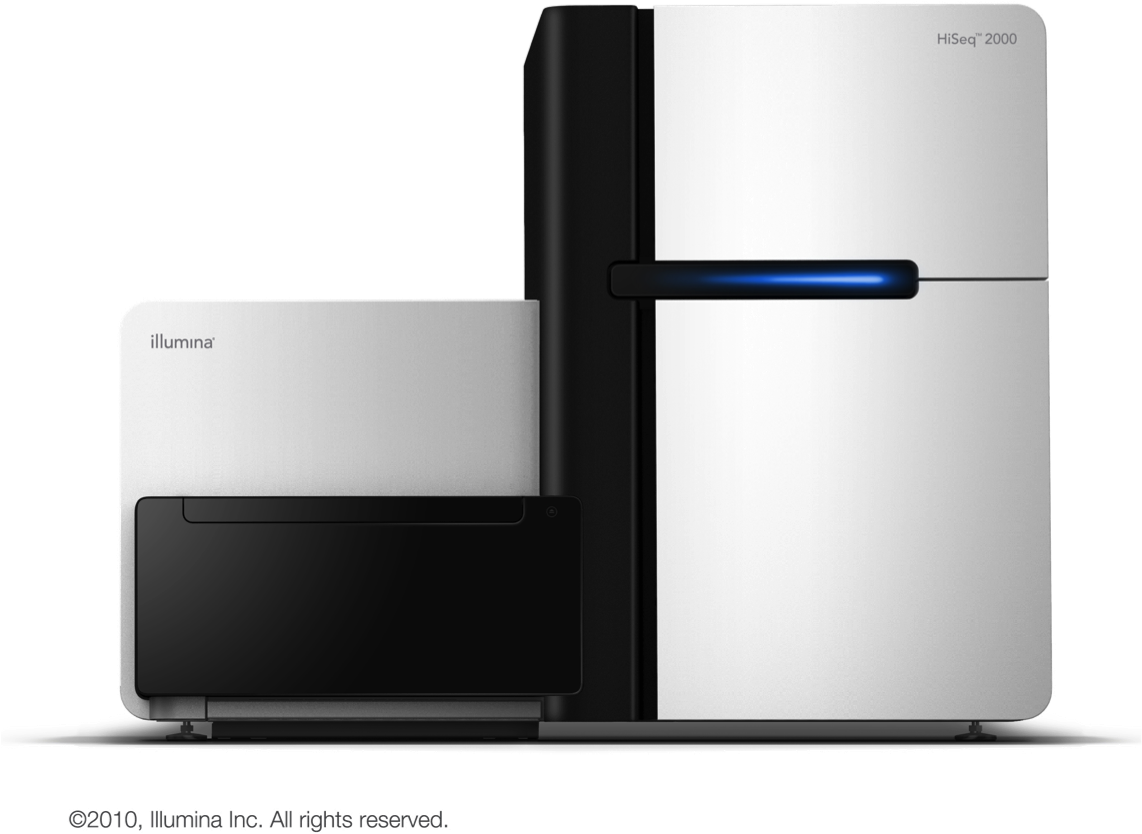
\includegraphics[width=0.7\textwidth]{images/illumina_hiseq}
  \end{center}  
\end{frame}

% Broad differences in chemistry and output
\begin{frame}
  \frametitle{Four different chemistries
\footnote{\tiny{Loman \textit{et al}. (2012) \textit{Nat. Rev. Micro.} \textbf{31}:294-296 \href{http://dx.doi.org/10.1038/nbt.2522}{doi:10.1038/nbt.2522
}}}
}
  Reads differ by technology, and can require different bioinformatic treatment$\ldots$
  \begin{itemize}
    \item \textcolor{hutton_green}{\textbf{Roche/454}: Pyrosequencing (long reads, but expensive, and high homopolymer errors) (700-800bp, 0.7Gbp, 23h)}
    \item \textcolor{hutton_blue}{\textbf{Illumina}: Reversible terminator (cost-effective, massive throughput, but short read lengths) (2x150bp, 1.5Gbp, 27h)}
    \item \textcolor{RawSienna}{\textbf{Ion Torrent}: Proton detection (short run times, good throughput, high homopolymers errors) (200bp, 1Gbp, 3h)}
    \item \textcolor{hutton_purple}{\textbf{PacBio}: Real-time sequencing (very long reads, high error rate, expensive) (3-15kbp, 3Gbp/day, 20min)}
  \end{itemize}
  $\ldots$ different error profiles, varying capability to assemble/determine variation
\end{frame}

% Sequencer relative costs
\begin{frame}
  \frametitle{Costs of sequencing\footnote{\tiny{Miyamoto \textit{et al}. (2014) \textit{BMC Genomics} \textbf{15}:699 \href{http://dx.doi.org/10.1186/1471-2164-15-699}{doi:10.1186/1471-2164-15-699}}}}
    \begin{center}
      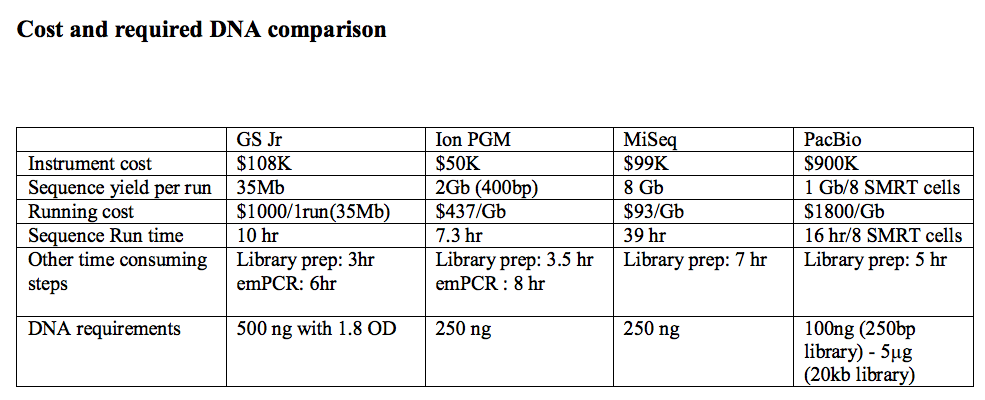
\includegraphics[width=1\textwidth]{images/miyamoto_costs}
    \end{center}      
\end{frame}

% How many genomes do we have, now?
\begin{frame}
  \frametitle{After that, the flood$\ldots$}
  High-throughput sequencing methods have completely changed the landscape of biology \\
  \textbf{(Nearly) complete, (mainly) accurate sequence data is now inexpensive} (and cheaper than analysis)
  \begin{itemize}
    \item \textcolor{hutton_green}{\href{http://www.genomesonline.org/cgi-bin/GOLD/index.cgi?page_requested=Complete+Genome+Projects&subset_requested=Complete+And+Published}{GOLD} (19/2/2014): 3,011 ``finished'' ; 9,891 ``permanent draft'' genomes}
    \item \textcolor{hutton_blue}{\href{http://www.genomesonline.org/cgi-bin/GOLD/index.cgi?page_requested=Complete+Genome+Projects&subset_requested=Complete+And+Published}{GOLD} (18/11/2014): 6,649 ``finished'' ; 23,552 ``permanent draft'' genomes}
    \item \textcolor{RawSienna}{\href{http://www.ncbi.nlm.nih.gov/Traces/wgs/}{NCBI WGS} (19/2/2014): 17,023 microbial genomes}
    \item \textcolor{hutton_purple}{\href{http://www.ncbi.nlm.nih.gov/Traces/wgs/}{NCBI WGS} (18/11/2014): 26,026 microbial genomes}
  \end{itemize}
\end{frame}

% And how many are we going to have?
\begin{frame}
  \frametitle{Predicting the future is hard$\ldots$}
    Su \textit{et al}. attempted to answer this\footnote{\tiny{\href{http://sulab.org/2013/06/sequenced-genomes-per-year/}{http://sulab.org/2013/06/sequenced-genomes-per-year/}}}:
    \begin{center}
      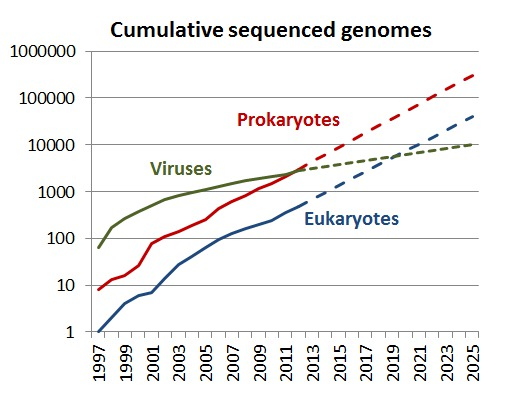
\includegraphics[width=0.5\textwidth]{images/cumulative_sequenced_genomes1}
      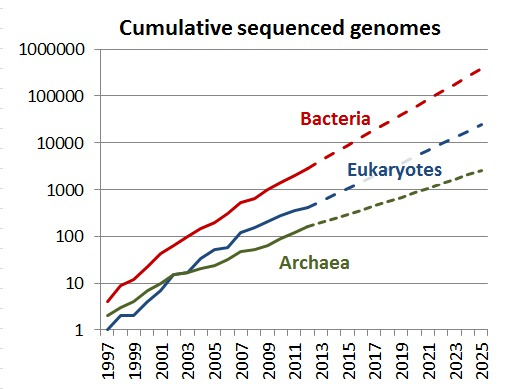
\includegraphics[width=0.5\textwidth]{images/cumulative_sequenced_genomes2}
    \end{center}     
%    How will we keep this much genomic data well-organised?
\end{frame}

% Nanopore
\begin{frame}
  \frametitle{What's coming next?}
  Oxford Nanopore. A sequencer the size of your hand.
    \begin{center}
      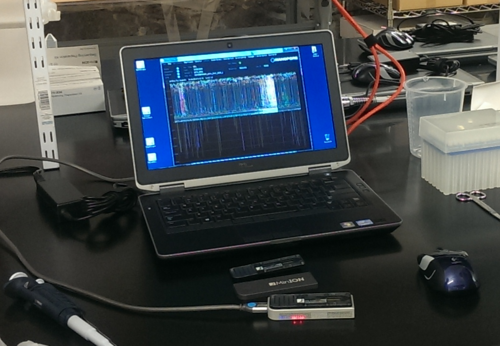
\includegraphics[width=0.48\textwidth]{images/minion_run}\thinspace
      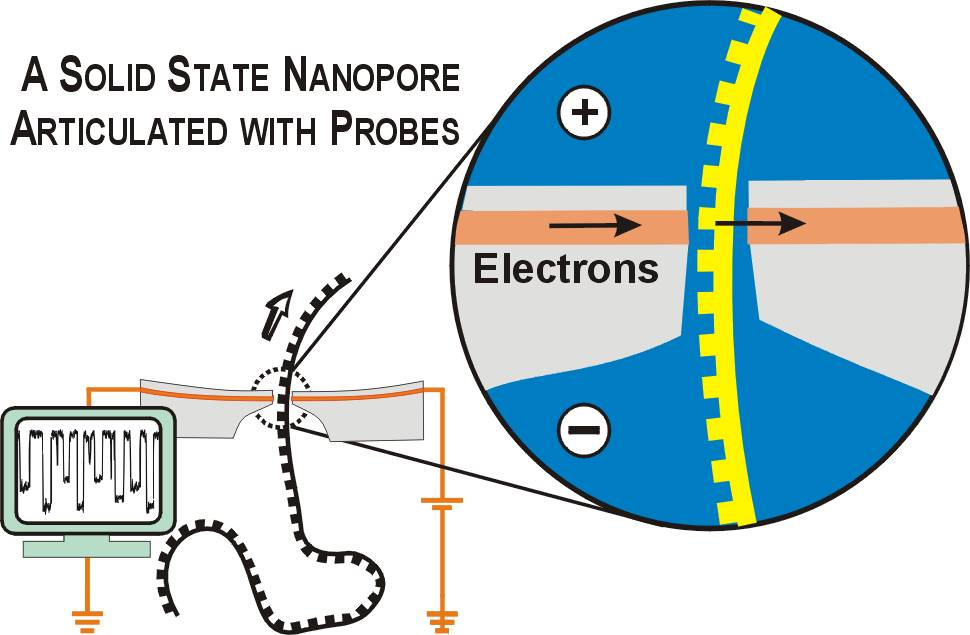
\includegraphics[width=0.48\textwidth]{images/nanopore_schematic}
    \end{center} 
    \begin{itemize}
      \item Microfluidics, single-molecule sequencing; 11-70kbp reads
      \item Reports current across pore (tiny electron microscope) as molecule moves through
      \item \$10/Mbp, 110Mbp per flowcell\footnote{\tiny{Yaniv Erlich (2013) \href{http://erlichya.tumblr.com/post/66376172948/hands-on-experience-with-oxford-nanopore-minion}{Future Continuous blog}}}
    \end{itemize}          
\end{frame}